% Linewatch executive summary (one page). Build: pdflatex executive-summary.tex (twice, for the header band)
% Numbers match the slide deck's results figure and docs/evaluation.md.
\documentclass[10pt]{article}
\usepackage[letterpaper,margin=0.55in,top=0.5in,bottom=0.45in]{geometry}
\usepackage[default]{sourcesanspro}
\usepackage[T1]{fontenc}
\usepackage{xcolor,graphicx,booktabs,enumitem,tikz,pgfplots,microtype,ragged2e,sansmath}
\usepackage[hidelinks]{hyperref}
\pgfplotsset{compat=1.17}

\definecolor{nv}{HTML}{5E8E1E}
\definecolor{nvlight}{HTML}{F2F6EA}
\definecolor{ink}{HTML}{1F2328}
\definecolor{muted}{HTML}{6B7280}
\definecolor{base}{HTML}{A3A3A3}
\definecolor{rule}{HTML}{DADFD4}
\color{ink}
\hypersetup{colorlinks,urlcolor=nv,linkcolor=nv}

\newcommand{\repo}{https://github.com/ALL-Applied-AI-Network/msoe-ai-club-rockwell-automation-nvidia-hackath-austin-koske-s-team-8e90f213c6}
\newcommand{\sect}[1]{\par\vspace{7pt}{\color{nv}\bfseries\footnotesize\MakeUppercase{#1}}\par\vspace{2pt}{\color{rule}\hrule height 0.5pt}\vspace{5pt}}
% One headline-number tile; four sit side by side under the intro.
\newcommand{\kpi}[3]{%
  \begin{tikzpicture}[baseline=(b.north)]
    \node[fill=nvlight,rounded corners=3pt,text width=0.238\textwidth-16pt,inner sep=8pt,minimum height=1.6cm,align=left,anchor=north] (b)
      {{\fontsize{20}{22}\selectfont\bfseries\color{nv}#1}\\[1pt]{\footnotesize\bfseries #2}\\[-2pt]{\scriptsize\color{muted}#3}};
  \end{tikzpicture}}
\setlist{leftmargin=1.05em,itemsep=2pt,topsep=2pt,parsep=0pt,label={\color{nv}\textbullet}}
\setlength{\parindent}{0pt}
\setlength{\parskip}{4pt}
\linespread{1.06}
\makeatletter\renewcommand\normalsize{\@setfontsize\normalsize{9.5}{11.5}}\makeatother

\begin{document}
\pagestyle{empty}\sansmath\RaggedRight

\begin{tikzpicture}[remember picture,overlay]
  \fill[nv] (current page.north west) rectangle ([yshift=-0.09in]current page.north east);
\end{tikzpicture}

% ---------- header ----------
{\fontsize{24}{26}\selectfont\bfseries Linewatch}\par\vspace{1pt}
{\large\color{muted} Recipe-aware inspection at the edge}\hfill{\footnotesize\color{muted}Rockwell Automation $\times$ NVIDIA Physical AI Hackathon $\cdot$ MSOE}\par
\vspace{3pt}
{\footnotesize Reagan Burkemper $\cdot$ Cameron Delpage $\cdot$ Hayden Fons $\cdot$ Zoe Kirkman $\cdot$ Srijan Kumar $\cdot$ Josiah Mathews $\cdot$ Alayna Ostler $\cdot$ Austin Koske}\par
\vspace{6pt}
Linewatch catches off-recipe vials while they are being filled. Using the station's existing cameras and the recipe order, it tells
the operator to scrap, flush or hold, with a deadline and a reason. It is trained only in simulation and runs on an NVIDIA GB10.\par
\vspace{8pt}

% ---------- headline numbers ----------
\noindent\kpi{76\%\,$\rightarrow$\,94\%}{carryover vials caught}{color check vs Linewatch}\hfill
\kpi{8 s}{fill end to the call}{median; 120\,s deadline, 100+\,s spare}\hfill
\kpi{0 s}{added per vial}{vs 20+\,s at CSI's sorter}\hfill
\kpi{\$10M}{average food recall}{caught at the fill instead}\par
\vspace{2pt}{\scriptsize\color{muted}Same 202 held-out synthetic carryover vials for both catch rates. Decision time: Run 5, every SCRAP before its vial reached the tray. Recall cost:
\href{https://www.food-safety.com/signature-series/recall-the-food-industrys-biggest-threat-to-profitability/}{FMI/GMA}.}\par

% ---------- two columns ----------
\noindent
\begin{minipage}[t]{0.475\textwidth}
\sect{The manufacturing problem}
CSI's Fluid Mixing Station 3 fills each vial by recipe from four dye tanks (clear, orange, yellow, blue; yellow was down for our tests); a conveyor and robot arm then
carry it to a sorter that drops it in a Good or Bad tray. Lines that run several recipes on shared equipment leave old product in the line at every changeover: \textbf{carryover}.
CSI's sorter is never told the order, so a vial of the previous recipe still passes as a valid color, and it stops every
vial for over 20\,s to say only pass or fail.

\vspace{2pt}
{\centering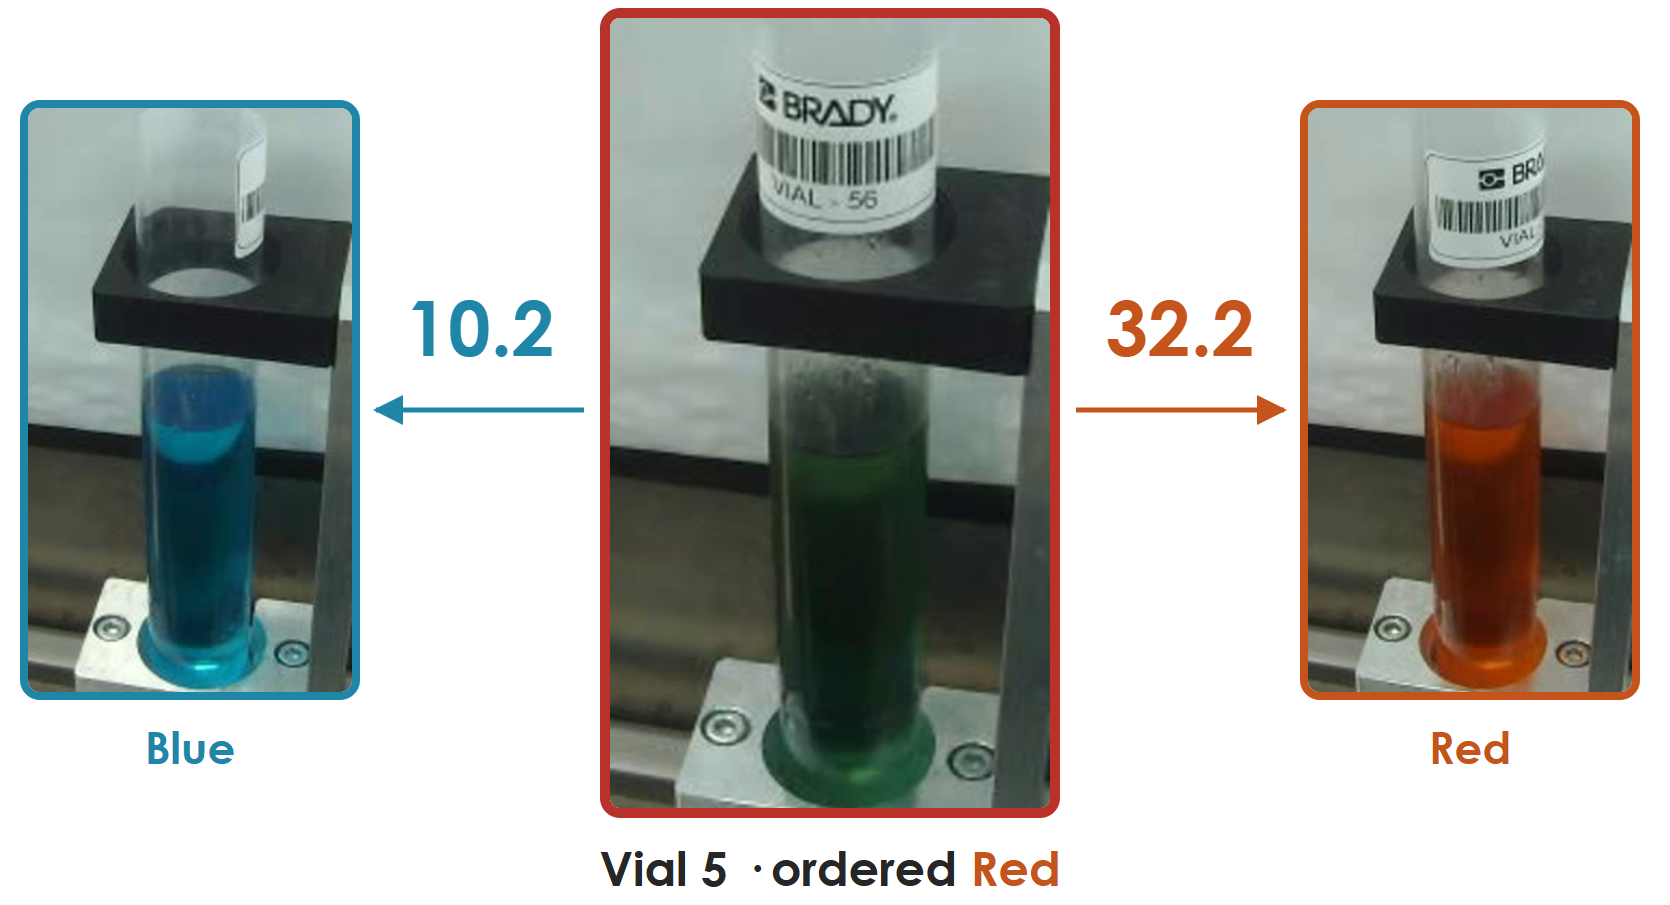
\includegraphics[width=0.42\linewidth]{vial5.png}\par\vspace{1pt}
{\scriptsize\color{muted}Vial 5 at CSI: red ordered, blue still in the line.}\par}

\sect{Technical approach}
\begin{enumerate}[label={\color{nv}\bfseries\arabic*}]
  \item \textbf{Perception.} A YOLO11n detector (COCO-pretrained) finds the vial; a temporal U-Net segments the liquid across
        consecutive frames as it fills. Both are trained only on Isaac Sim renders.
  \item \textbf{Measurement QA.} Glare, clipping, too few liquid pixels or an unstable track give \emph{can't verify}, never a guess.
  \item \textbf{Spec check.} The fill-end color is compared with one reference vial of the ordered recipe: more than $\Delta E_{00}$\,5 away is out of spec ($\Delta E_{00}$ is the standard color-difference measure; 5 is clearly visible side by side).
  \item \textbf{Carryover.} If the shift points toward the previous recipe (cosine of at least 0.75 in Lab or optical density, where dyes mix
        linearly), the cause is carryover.
  \item \textbf{Action.} SCRAP before the sorter (120\,s deadline), FLUSH before the next fill, STOP after 3 deviations, or HOLD.
        Nemotron words the explanation; the rules decide. Our rule explainer matched the evidence on 20/20 vials, Cosmos-Reason1 on 6--9/20.
\end{enumerate}

\sect{How we used the CSI equipment}
\begin{itemize}
  \item Ran on \textbf{CSI's GB10} with the station's \textbf{fill and tray cameras}: 3 visits (5\,h) of integration testing,
        then final runs (4 blue vials, then 4 red).
\end{itemize}
\end{minipage}\hfill
\begin{minipage}[t]{0.475\textwidth}
\sect{How we use Physical AI}
\begin{itemize}
  \item \textbf{Sim-to-real:} trained on Isaac Sim renders of the station's twin, run on CSI's real cameras.
  \item \textbf{Synthetic data:} 14,400 carryover renders on NVIDIA Brev set the thresholds.
  \item \textbf{Edge AI:} 86\,ms per frame on the GB10; 0 of 50,941 frames dropped live.
  \item \textbf{Bring your own line:} new recipe, one reference vial (no retraining); new station, a config file
        and a short tray video; new product, render its twin and retrain.
\end{itemize}

\sect{Evidence that it works}
{\footnotesize\bfseries Out-of-spec vials caught on 1,195 held-out changeovers}\par\vspace{2pt}
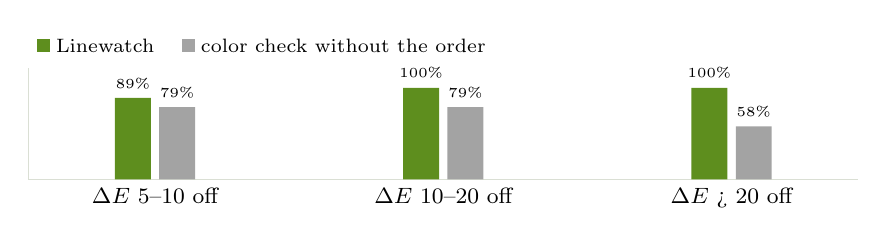
\begin{tikzpicture}
\begin{axis}[
  width=\linewidth, height=3.0cm, ybar=3pt, bar width=13pt, ymin=0, ymax=122, axis lines*=left,
  axis line style={rule}, ytick=\empty, symbolic x coords={a,b,c}, xtick=data,
  xticklabels={{$\Delta E$ 5--10 off},{$\Delta E$ 10--20 off},{$\Delta E$ > 20 off}},
  enlarge x limits=0.22, xticklabel style={font=\footnotesize}, major tick length=0pt,
  nodes near coords={\pgfmathprintnumber{\pgfplotspointmeta}\%}, nodes near coords style={font=\tiny},
  every axis plot/.append style={draw=none},
  legend style={font=\scriptsize,draw=none,fill=none,at={(0,1.0)},anchor=south west,legend columns=2,/tikz/every even column/.append style={column sep=8pt}},
  legend image code/.code={\fill (0cm,-0.06cm) rectangle (0.17cm,0.11cm);}]
\addplot[fill=nv] coordinates {(a,89) (b,100) (c,100)};
\addplot[fill=base] coordinates {(a,79) (b,79) (c,58)};
\legend{Linewatch, color check without the order}
\end{axis}
\end{tikzpicture}\par
{\scriptsize\color{muted}The color check gets \emph{worse} on big shifts: they look like another valid recipe.}\par

\vspace{6pt}
{\footnotesize
\setlength{\tabcolsep}{2pt}\renewcommand{\arraystretch}{1.22}
\begin{tabular*}{\linewidth}{@{}l@{\extracolsep{\fill}}cccc@{}}
\toprule
 & \textbf{Synthetic} & \textbf{Run 5 +} & \textbf{Run 5} & \textbf{CSI} \\[-3pt]
 & {\scriptsize\color{muted}held-out} & {\scriptsize\color{muted}carryover added} & {\scriptsize\color{muted}as recorded} & {\scriptsize\color{muted}final run} \\
\midrule
Out-of-spec caught & 189/202 & 5/5 & 7/11 & \textbf{4/4} \\
False scraps & 4.3\% (43/993) & 1/16 & 0/9 & \textbf{0/4} \\
Baseline caught & 154/202 & 5/5 & 6/11 & 4/4 \\
SCRAP before the tray & -- & -- & 9/9 & \textbf{4/4} \\
\bottomrule
\end{tabular*}}\par
{\scriptsize\color{muted}Run 5 is the organizers' 30-vial run; \emph{carryover added} recolors its real footage with known amounts. Baseline: accepts any vial within $\Delta E$ 5 of a known recipe, without the order.}

\sect{How we scored it}
\textbf{Truth is the spec:} a vial is out of spec when its true color, the optical-density mix of the clean and previous
recipes at the true residue, is more than $\Delta E_{00}$ 5 from the order. Measured colors get camera noise matched to Runs 1--4.
Thresholds were chosen on training scene families and reported once on held-out ones; Run 5 was scored once with settings frozen.\par
\textbf{Limits:} misses sit within camera noise of the line; vials with too little visible liquid get no call; sorting needs PLC access.
\end{minipage}

\vfill
{\color{rule}\hrule height 0.5pt}\vspace{4pt}
{\footnotesize
\textbf{Code} \href{\repo}{GitHub repository} \quad
\textbf{Results} \href{\repo/blob/main/docs/evaluation.md}{evaluation.md} \quad
\textbf{Design} \href{\repo/blob/main/docs/architecture.md}{architecture.md} \quad
\textbf{Data} \href{\repo/blob/main/docs/data.md}{data.md} \quad
\textbf{Sources} \href{\repo/blob/main/docs/industry-research.md}{industry-research.md} \quad
\textbf{Video} \href{https://youtu.be/byBT2FvAK1E}{youtu.be/byBT2FvAK1E}\par}

\end{document}
